\section{两个随机变量的函数的分布}

我们先来看一个问题: $X,Y$是相互独立的离散型随机变量, 等概率地取$[0,3]$区间的整数. 问$X+Y=3$的概率是多少? 

解答也不难. 考虑一共有$(0, 3), (1, 2), (2, 1), (3, 0)$四种情况, 相加即可. 那么我们把这个$X+Y$看做新的随机变量, 应该如何求? 实际上我们只要枚举就好了.
$$
\begin{aligned}
P_W(w) & =P(X+Y=w) \\
& =\sum_x P(X=x)  P(Y=w-x) \\
& =\sum_x P_X(x) P_Y(w-x) . 
\end{aligned}
$$

我们现在来系统的考察对于任意的分布函数, 几个常见的两个随机变量参与运算之后的概率密度. 

\paragraph{(一) $Z=X+Y$ 的分布}

设 $(X, Y)$ 是二维连续型随机变量, 它具有概率密度 $f_{X,Y}(x, y)$.那么连续型随机变量$Z=X+Y$的概率密度是多少?

大致思路: 
    \begin{itemize}
        \item 先来求 $Z=X+Y$ 的分布函数 $F_Z(z)$
        \item $F_Z(z)=P(Z \leq z)=\iint_{x+y \leq z} f_{X,Y}(x, y) \mathrm{d} x \mathrm{~d} y$
    \end{itemize}
    $$\begin{aligned}
        F_Z(z)&=\int_{-\infty}^{\infty}\left[\int_{-\infty}^{\purple {z-y}} f({\red{x}}, y) \mathrm{d} {\red{x}}\right] \mathrm{d} y \\ 
        &\stackrel{{\red x}:=\teal{u-y}}{\stackrel{\rule{1.5cm}{0.4pt}}{\rule{1.5cm}{0.4pt}}}
        \int_{-\infty}^{\infty}\left[\int_{-\infty}^z f({\teal {u-y}}, y) \mathrm{d} u\right] \mathrm{d} y\\
        &=\int_{-\infty}^z\left[\int_{-\infty}^{\infty} f(u-y, y) \mathrm{d} y\right] \mathrm{d} u
    \end{aligned}$$

    这里的换元法实际上是使用给定的不等关系$x+y\leq z$为了消去$x$, 减少变量个数. 

    根据定义, 求导得到: 
    $f_{X+Y}(z)=\int_{-\infty}^{\infty} f(u-y, y) \mathrm{d} y=\int_{-\infty}^{\infty} f(z-y, y) \mathrm{d} y.$

我们用定理的形式总结这一事实: 
\begin{theorem}
    设 $(X, Y)$ 是二维连续型随机变量, 它具有概率密度 $f_{X,Y}(x, y)$. 则 $Z=X+Y$ 仍为连续型随机变量, 其概率密度为
    $$f_{X+Y}(z)=\int_{-\infty}^{\infty} f(z-y, y) \mathrm{d} y$$
    或
    $$
f_{X+Y}(z)=\int_{-\infty}^{\infty} f(x, z-x) \mathrm{d} x
$$
\end{theorem}

如果$X,Y$相互独立的话, 上述公式可以进一步地写作
\begin{itemize}
    \item $f_{X+Y}(z)=\int_{-\infty}^{\infty} f_X(z-y) f_Y(y) \mathrm{d} y$;
    \item $f_{X+Y}(z)=\int_{-\infty}^{\infty} f_X(x) f_Y(z-x) \mathrm{d} x$
\end{itemize}

\begin{asidebox}
    卷积: 刚刚常见的操作其实有一个名字: 卷积. 比如我们在求两个多项式的乘积的时候, $(\sum_{i=0}^{\infty} a_i x^i)(\sum_{j=0}^{\infty} b_j x^j).$

    我们可以用这样的公式计算: 

    $$
    \begin{aligned}
        \sum_{k=0}^{\infty}\left(\sum_{i+j=k} a_i b_j\right) x^k
        =\sum_{k=0}^{\infty}\left(\sum_{i=0}^k a_i b_{k-i}\right) x^k
    \end{aligned}
    $$

    刚刚的那个问题同样和这个问题有类似的性质, 只是求和号变为了积分号. 

\end{asidebox}

为了方便起见, 这两个公式称为 $f_X$ 和 $f_Y$ 的卷积公式, 记为 $f_X * f_Y$, 即
$$
f_X * f_Y=\int_{-\infty}^{\infty} f_X(z-y) f_Y(y) \mathrm{d} y=\int_{-\infty}^{\infty} f_X(x) f_Y(z-x) \mathrm{d} x
$$

\begin{asidebox}
    直观理解卷积: 先把纸片翻一下, 然后平移, 最后对应相乘相加. 如\cref{fig:convolution}.
\end{asidebox}

\begin{figure}
    \center
    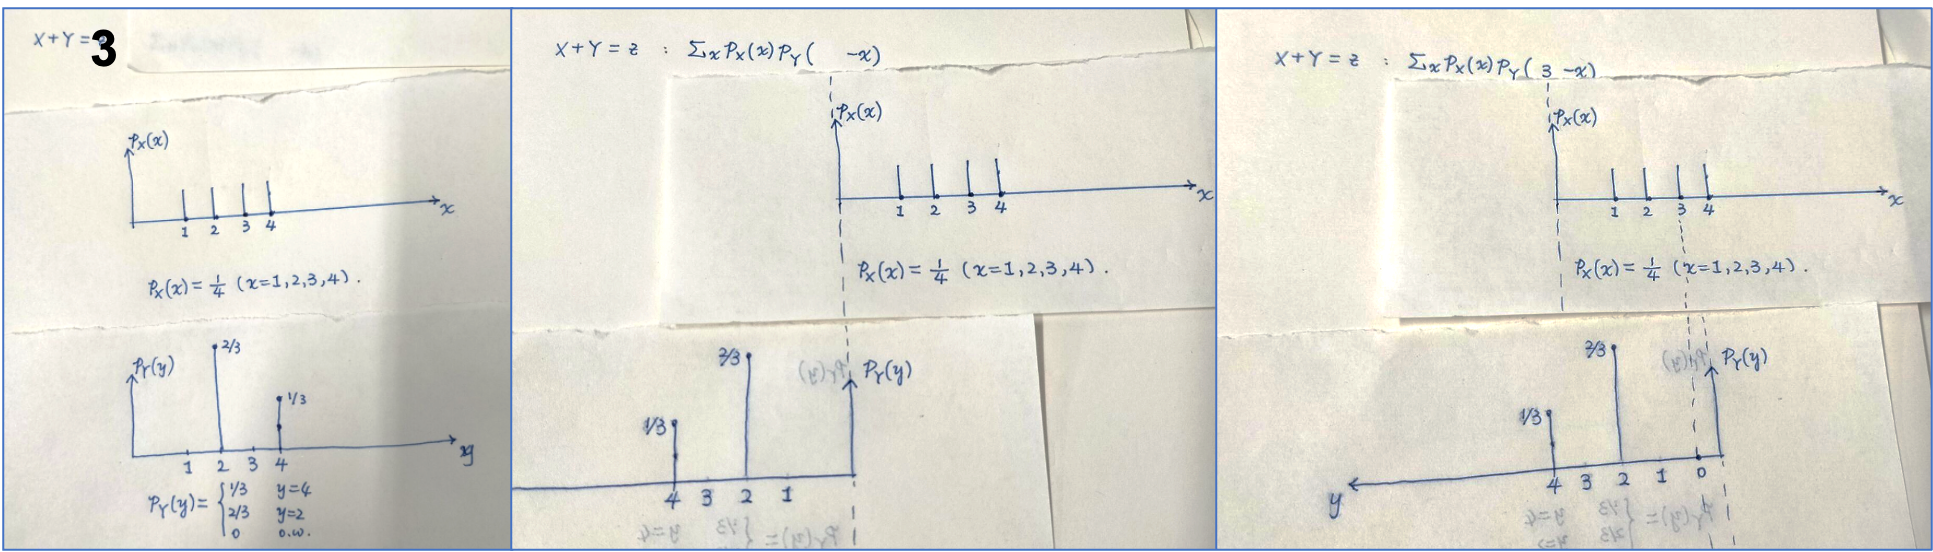
\includegraphics[width=\textwidth]{fig/ch3/convolution.png}
    \caption{直观理解卷积}
    \label{fig:convolution}
\end{figure}

\paragraph{(二)$Z=Y/X,Z=XY$的分布}

设 $(X, Y)$ 是二维连续型随机变量, 它具有概率密度 $f_{X,Y}(x, y)$.连续型随机变量$Z=Y/X$的概率密度是多少?

我们还是还是首先设出$F_{Y/X}(z)=P(Y/X\leq z)$. 但是这里由于函数的不连续性, 需要分两种情况: $x<0, x>0$分别考虑:

$$
\begin{aligned}
F_{Y / X}(z) & =P(Y / X \leq z)=\iint_{\stackrel{y / x \leq z}{x<0}} f(x, y) \mathrm{d} y \mathrm{~d} x+\iint_{\stackrel{y / x \leq z}{x>0}} f(x, y) \mathrm{d} y \mathrm{~d} x \\
& =\int_{-\infty}^0\left[\int_{z x}^{\infty} f(x, y) \mathrm{d} y\right] \mathrm{d} x+\int_0^{\infty}\left[\int_{-\infty}^{z x} f(x, y) \mathrm{d} y\right] \mathrm{d} x \\
& \varsub{y:=xu}{1cm} \int_{-\infty}^0\left[\int_z^{-\infty} x f(x, x u) \mathrm{d} u\right] \mathrm{d} x+\int_0^{\infty}\left[\int_{-\infty}^z x f(x, x u) \mathrm{d} u\right] \mathrm{d} x \\
& =\int_{-\infty}^0\left[\int_{-\infty}^z(-x) f(x, x u) \mathrm{d} u\right] \mathrm{d} x+\int_0^{\infty}\left[\int_{-\infty}^z x f(x, x u) \mathrm{d} u\right] \mathrm{d} x \\
& =\int_{-\infty}^z\left[\int_{-\infty}^+\infty|x| f(x, x u) \mathrm{d} u\right] \mathrm{d} x
\end{aligned}
$$

遵循同样的模式, 同样可以求出: $Z=XY$的概率分布. 
$$
\begin{aligned} & F_{XY}(z)=P(XY\leq z)\\
 & =\iint_{\substack{xy\leq z\\
 x<0}}f(x,y)\dd y\dd x+\iint_{\substack{xy\leq z\\
 x>0}}f(x,y)\dd y\dd x\\
 & =\int_{-\infty}^{0}\left(\int_{z/x}^{+\infty}f(x,y)\dd y\right)\dd x+\int_{0}^{+\infty}\left(\int_{-\infty}^{z/x}f(x,y)\dd y\right)\dd x\\
 & \varsub{y:=u/x}{1.5cm}\int_{-\infty}^{0}\left(\int_{z/x}^{+\infty}f\left(x,\frac{u}{x}\right)d\left(\frac{u}{x}\right)\right)\dd x+\int_{0}^{+\infty}\left(\int_{-\infty}^{z/x}f\left(x,\left(\frac{u}{x}\right)\dd x\right)\right)\\
 & =\int_{-\infty}^{0}\left(\left(\frac{1}{x}\right)\int_{z}^{-\infty}f\left(x,\frac{u}{x}\right)\dd u\right)\dd x+\int_{0}^{+\infty}\left(\frac{1}{x}\int_{-\infty}^{z}f\left(x,\frac{u}{x}\right)\dd u\right)\dd x\\
 & =\int_{0}^{z}\left(\int_{-\infty}^{\infty}\frac{1}{|x|}f\left(x,\frac{u}{x}\right)\dd u\right)\dd x
\end{aligned}
$$

\paragraph{(三) $M=\min \{X, Y\}$的分布}

$X, Y$ 是两个\emph{相互独立}的随机变量, 它们的分布函数分别为 $F_X(x)$ 和$F_Y(y)$.求 $M=\min \{X, Y\}$的分布函数.


   $$
\begin{aligned}
F_{\min }(z) & =P(N \leq z\}=1-P\{N>z) \\
& =1-P(X>z, Y>z\}=1-P(X>z) \cdot P\{Y>z)
\end{aligned}
$$

也就是
$$
F_{\min }(z)=1-\left[1-F_X(z)\right]\left[1-F_Y(z)\right] .
$$

上述的三个情况都可以推广到$n$维的情形.